\chapter{Implementarea}

În acest capitol va fi prezentata implementarea bibliotecii software pentru dezvoltarea de algoritmi și aplicații de recunoaștere a obiectelor.

Biblioteca a fost implementata într-un mod hibrid.
Interfețele au fost definite în limbajul C++, iar implementările au fost făcute atât în C++ cat și în Python.
Biblioteca a fost scrisa și testata cu Visual Studio 2013.


Structura de directoare a bibliotecii este:
\verbatiminput{treeview.txt}
Fiecare pachet este situat in propriul director.
Declaratiile se gasesc in directorul "\verb!include!"
, iar implementarile in "\verb!src!".

\pagebreak
\section{Diagrama de clase}

\subsection{Core}
Pachetul "core" conține interfețe de baza ale bibliotecii.
\begin{figure}[H]
	\centering
		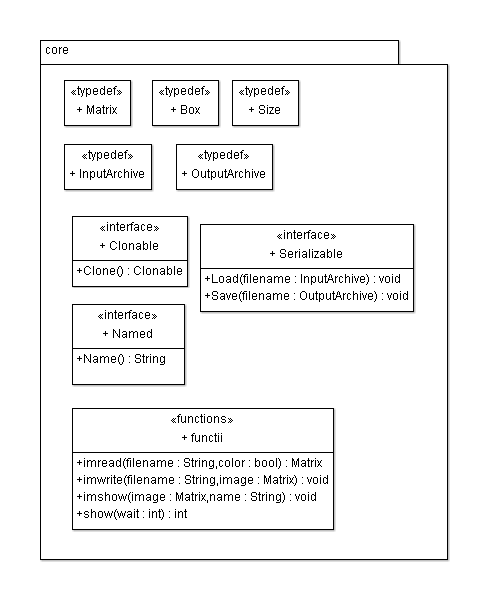
\includegraphics[width=0.95\textwidth]{uml/coreClassDiagram.png}
	\caption{core Class Diagram}
	\label{fig:coreClassDiagram}
\end{figure}

\subsection{Dataset}
%[TODO:] Discutie depre PASCAL VOC, ImageNet etc.


Pachetul "dataset" conține clase care modelează baza de date pentru antrenament și implementează funcționalități de importare unor formate uzuale.
\begin{figure}[H]
	\centering
	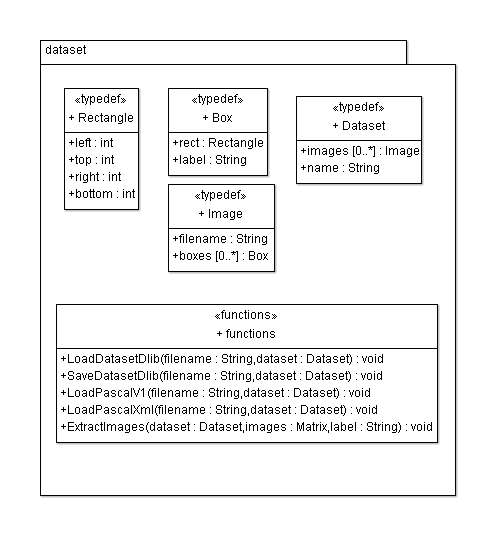
\includegraphics[width=1.0\textwidth]{uml/datasetClassDiagram.png}
	\caption{Diagrama de clase: dataset}
	\label{fig:datasetClassDiagram}
\end{figure}

\subsection{Image Pyramid}
Pachetul "image-pyramid" conține interfețe și implementări care servesc la construcția piramidei de imagini.
\begin{figure}[H]
	\centering
	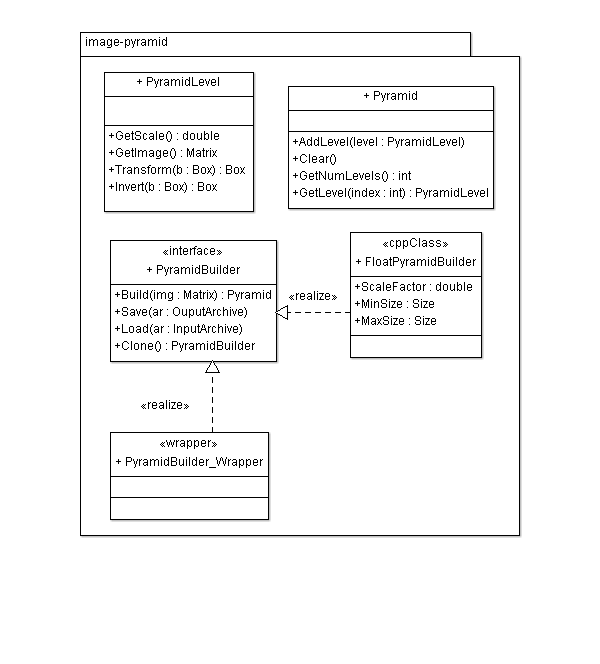
\includegraphics[width=1.00\textwidth]{uml/imagepyramidClassDiagram.png}
	\caption{Diagrama de clase: image-pyramid}
	\label{fig:imagepyramidClassDiagram}
\end{figure}


Clasa FloatPyramidBuilder construiește o piramida de imagini folosind ScaleFactor ca factor de scalare și MinSize, MaxSize drept criterii de terminare.

Metodele Transform și Invert din clasa PyramidLevel transforma coordonate din spațiul imaginii sursa în cel al nivelului, respectiv invers.

\subsection{Image Scanning}
Pachetul "image-scanning" conține interfețe și implementări care servesc la scanarea imaginilor
\begin{figure}[H]
	\centering
		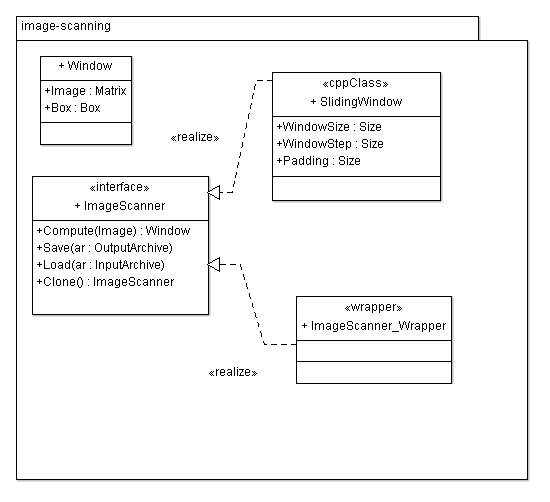
\includegraphics[width=1.00\textwidth]{uml/imagescanningClassDiagram.png}
	\caption{Diagrama de clase: image-scanning}
	\label{fig:imagescanningClassDiagram}
\end{figure}

\pagebreak
\subsection{Feature Extraction}
Pachetul "feature-extraction" conține interfețe și implementări care servesc la extragerea de trăsături din imagini.
\begin{figure}[H]
	\centering
		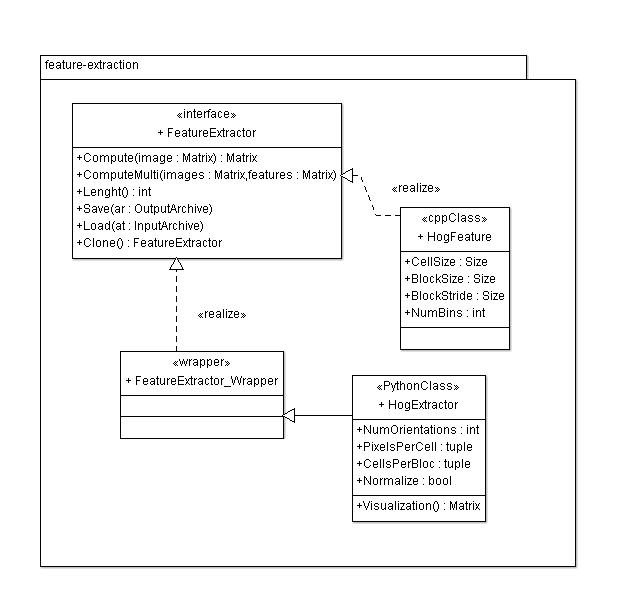
\includegraphics[width=1.00\textwidth]{uml/featureextractionClassDiagram.png}
	\caption{Diagrama de clase: feature-extraction}
	\label{fig:featureextractionClassDiagram}
\end{figure}

\pagebreak
\subsection{Classification}
Pachetul "classification" conține interfețe și implementări care servesc la clasificare și antrenarea clasificatorilor.
\begin{figure}[H]
	\centering
	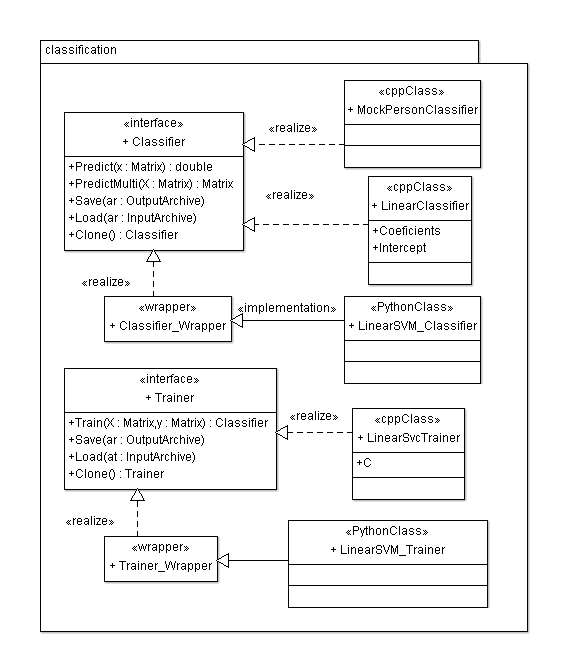
\includegraphics[width=1.00\textwidth]{uml/classificationClassDiagram.png}
	\caption{Diagrama de clase: classification}
	\label{fig:classificationClassDiagram}
\end{figure}

\subsection{Non Maxima Suppression}
Pachetul "non-maxima-suppression" conține interfețe și implementări care servesc la post-procesarea rezultatelor.
\begin{figure}[H]
	\centering
		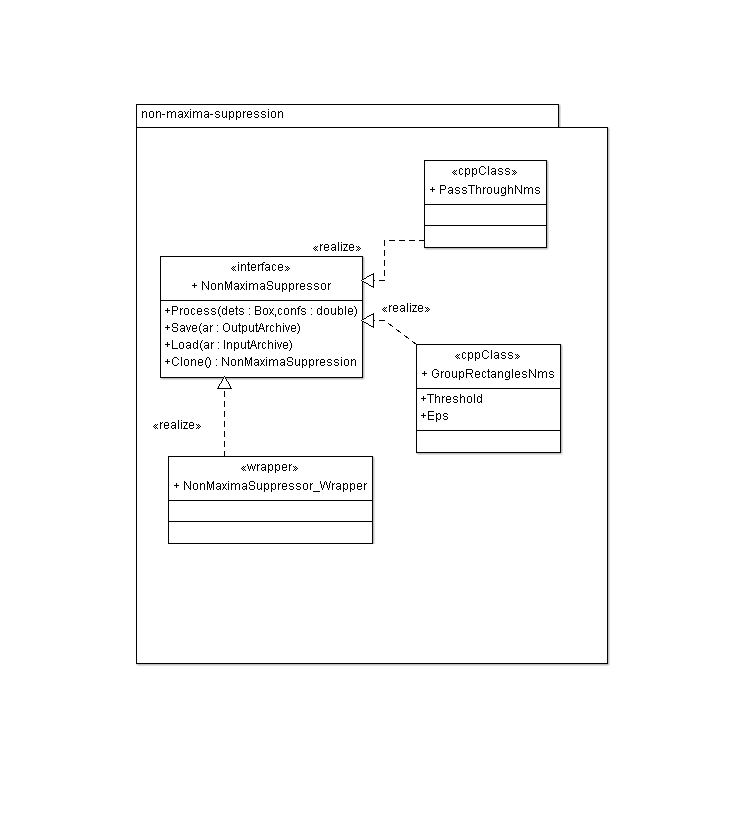
\includegraphics[width=1.00\textwidth]{uml/nonmaximasuppressionClassDiagram.png}
	\caption{Diagrama de clase: non-maxima-suppression}
	\label{fig:nonmaximasuppressionClassDiagram}
\end{figure}

\subsection{Detection}
Pachetul "detection" conține interfețe și implementări care servesc la recunoasterea obiectelor in imagini si la antrenarea algoritmilor.
\begin{figure}[H]
	\centering
		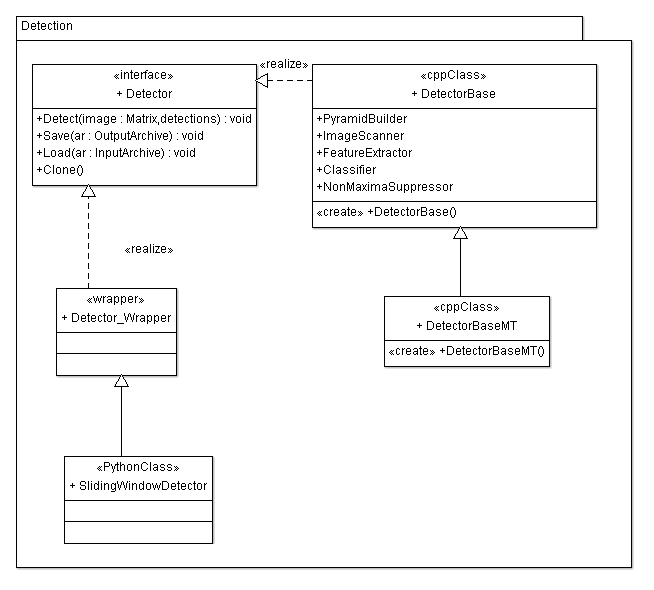
\includegraphics[width=1.00\textwidth]{uml/detectionClassDiagram.png}
	\caption{Diagrame de clase: detection}
	\label{fig:detectionClassDiagram}
\end{figure}
\begin{figure}[H]
	\centering
		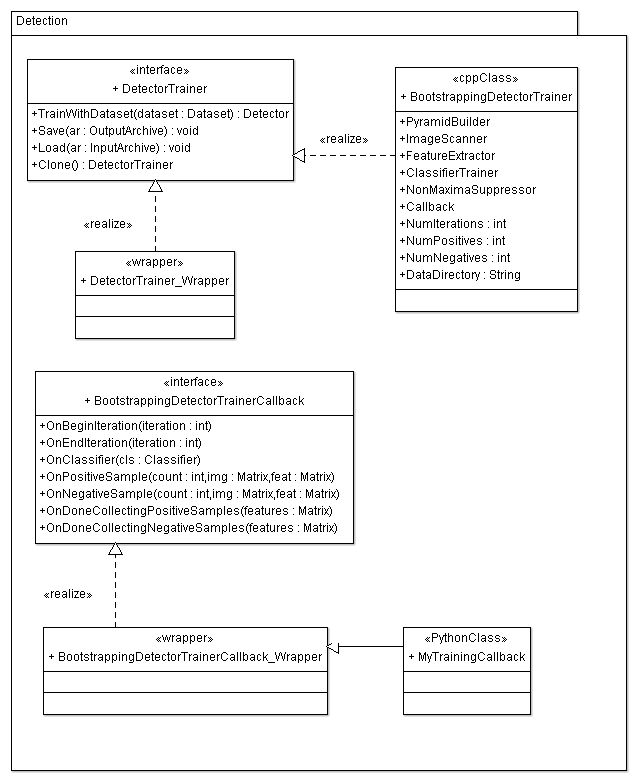
\includegraphics[width=1.00\textwidth]{uml/detection2ClassDiagram.png}
	\caption{Diagrama de clase: detection}
	\label{fig:detection2ClassDiagram}
\end{figure}

\pagebreak
\subsection{Python}
Pachetul "python" conține suportul necesar pentru interoperabilitatea cu limbajul Python.


\begin{figure}[H]
	\centering
		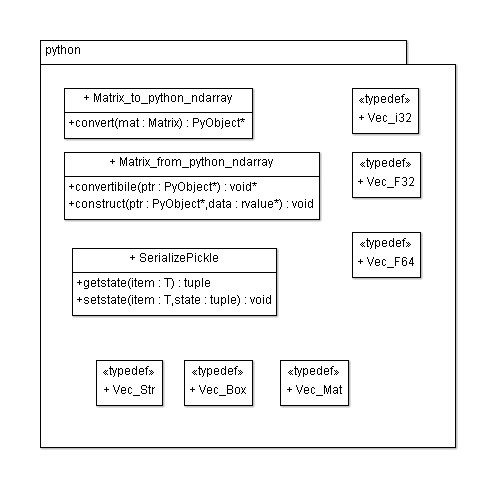
\includegraphics[width=1.00\textwidth]{uml/PythonClassDiagram.png}
	\caption{Diagrama de clase python}
	\label{fig:PythonClassDiagram}
\end{figure}




\pagebreak
\section{Algoritm de recunoaștere a persoanelor}

Cu ajutorul bibliotecii descrise în lucrare am implementat algoritmul de recunoaștere a personalelor în imagini descris în lucrarea "Histograms of Oriented Gradients for Human Detection", scrisa de Navneet Dalal și Bill Triggs\cite{Dalal05histogramsof}.
Acesta lucrare a introdus și descris extragerea trăsăturilor de imagine: histograma de gradienți orientați.

Pentru implementarea algoritmului s-au folosit următoarele componente:
\begin{itemize}
	\item Parcurgerea imaginii: FloatPyramidBuilder și SlidingWindow
	\item Extragerea de trăsături: HogFeature
	\item Clasificare: LinearSVM\_Classifier și LinearSVM\_Trainer
	\item Post-procesare: GroupRectanglesNms
	\item Baza de date: Dataset
	\item Antrenament: BootstrappingDetectorTrainer
\end{itemize}

Setul de imagini folosit pentru antrenarea algoritmului este cel oferit de institutul Inria\footnote{\url{http://www.inria.fr/centre/grenoble}} și poate fi descarcat gratuit de pe pagina web: \url{http://pascal.inrialpes.fr/data/human/}. 
Sunt oferite imagini și adnotări în formatul PASCAL VOC\footnote{\url{http://pascallin.ecs.soton.ac.uk/challenges/VOC/}}.
Datele conțin exemplare pozitive și negative.
%\section{Interoperabilitatea cu Python}
Interoperabilitatea cu limbajul Python se poate realiza folosind una dinte aceste tehnologii:
\begin{itemize}
	\item Python C Api\cite{pythonCAPI}
	\item SWIG\cite{swig}
	\item pyrex\cite{pyrex}
	\item ctypes\cite{ctypes}
	\item SIP\cite{sip}
	\item Boost.Python\cite{boostpython}
\end{itemize}

Am ales sa rezolv problema de interoperabilitate cu limbajul Python prin intermediul bibliotecii Boost.Python.
Particularitățile acestei biblioteci vor fi discutate în capitolul "Tehnologii folosite".

Pentru ca o clasa abstracta declarata în C++ sa poate fi implementata in Python, iar aceasta implementare sa fie disponibila atât în Python cat și în C++ este nevoie de o clasa ajutătoare care sa acționeze ca o legătura intre cele doua limbaje. 
Aceasta clase se implementează prin moștenire din clasa pe care dorim sa o expunem și clasa "wrapper" din Boost.Python.
O astfel de implementare poate fi observata in codul urmator:
\begin{lstlisting}[language=C++]
namespace object_recognition_toolkit
{
	namespace pyramid
	{
		namespace bp = boost::python;

		struct PyramidBuilder_Wrapper : public PyramidBuilder
			, public bp::wrapper < PyramidBuilder > {
			
			virtual ~PyramidBuilder_Wrapper() {}

			Pyramid Build(core::Matrix const& image) const
			{ return this->get_override("Build")(image); }

			boost::shared_ptr<PyramidBuilder> Clone() const
			{ return this->get_override("Clone")(); }
		};
	}
}
\end{lstlisting}

Pe urma, acesta clasa trebuie înregistrată pentru a fi vizibila în Python.
Înregistrarea se face cu Boost.Python prin intermediul clasei \verb!class_! după cum se observa mai jos:

\begin{lstlisting}[language=C++]
void py_regiser_pyramid()
{
using namespace boost::python;
using namespace object_recognition_toolkit::core;
using namespace object_recognition_toolkit::pyramid;
using object_recognition_toolkit::python_ext::serialize_pickle;

class_<PyramidLevel>("PyramidLevel", 
		init<const Matrix&, double>((arg("image"),arg("scale"))))
	.def("GetScale", &PyramidLevel::GetScale)
	.def("GetImage", &PyramidLevel::GetImage, 
		return_value_policy<copy_const_reference>())
	.def("Transform", &PyramidLevel::Transform<int>, arg("box"))
	.def("Invert", &PyramidLevel::Invert<int>, arg("box"))
	;

class_<Pyramid>("Pyramid", init<>())
	.def("AddLevel", &Pyramid::AddLevel, arg("level"))
	.def("Clear", &Pyramid::Clear)
	.def("GetNumLevels", &Pyramid::GetNumLevels)
	.def("GetLevel", &Pyramid::GetLevel, arg("index"), 
		return_value_policy<copy_const_reference>())
	;

class_<PyramidBuilder_Wrapper, boost::noncopyable>("PyramidBuilder")
	.def("Clone", pure_virtual(&PyramidBuilder::Clone))
	.def("Build", pure_virtual(&PyramidBuilder::Build), arg("image"))
	.enable_pickling()
	;
register_ptr_to_python<boost::shared_ptr<PyramidBuilder>>();

class_<FloatPyramidBuilder, bases<PyramidBuilder>>("FloatPyramidBuilder", init<>())
	.def(init<double, Size, Size>(args("scale_factor", "min_size", "max_size")))
	.def_readwrite("scale_factor", &FloatPyramidBuilder::scaleFactor_)
	.def_readwrite("max_size", &FloatPyramidBuilder::maxSize_)
	.def_readwrite("min_size", &FloatPyramidBuilder::minSize_)
	.def_pickle(serialize_pickle<FloatPyramidBuilder>())
	;
}
\end{lstlisting}

După care, implementarea aceste clase poate fi observata in codul urmator:
\begin{lstlisting}[language=Python,frame=single]
import object_recognition_toolkit as ort

class MyPyramidBuilder(ort.PyramidBuilder):

    def __init__(self, num):
        ort.PyramidBuilder.__init__(self)
        self.num = num
        
    def Build(self, image):
        pyr = ort.Pyramid()
        for si in range(self.num):
        	scale = 1.0//(2.0**float(si))
        	level = ort.PyramidLevel(image, scale)
            pyr.AddLevel(levele)
        return pyr
    
    #implement pickle support
    def __reduce__(self):
        initargs = (self.num, )
        # this is not necesary, becouse num is an init arg, 
        # but for the sake of example :)
        state = {'num': self.num} 
        return (MyPyramidBuilder, initargs, state, )
    
    def __setstate__(self, state):
        self.num = state['num']
\end{lstlisting}

Înainte de antrenare imaginile exemplarelor pozitive au fost decupate și redimensionate la o mărime de 64 pixeli lățime și 128 pixeli înălțime.
Exemplarele negative au fost folosite în întregime(fig. \ref{fig:exemplare_pozitive_inria_person}).

\begin{figure}[H]
	\centering
		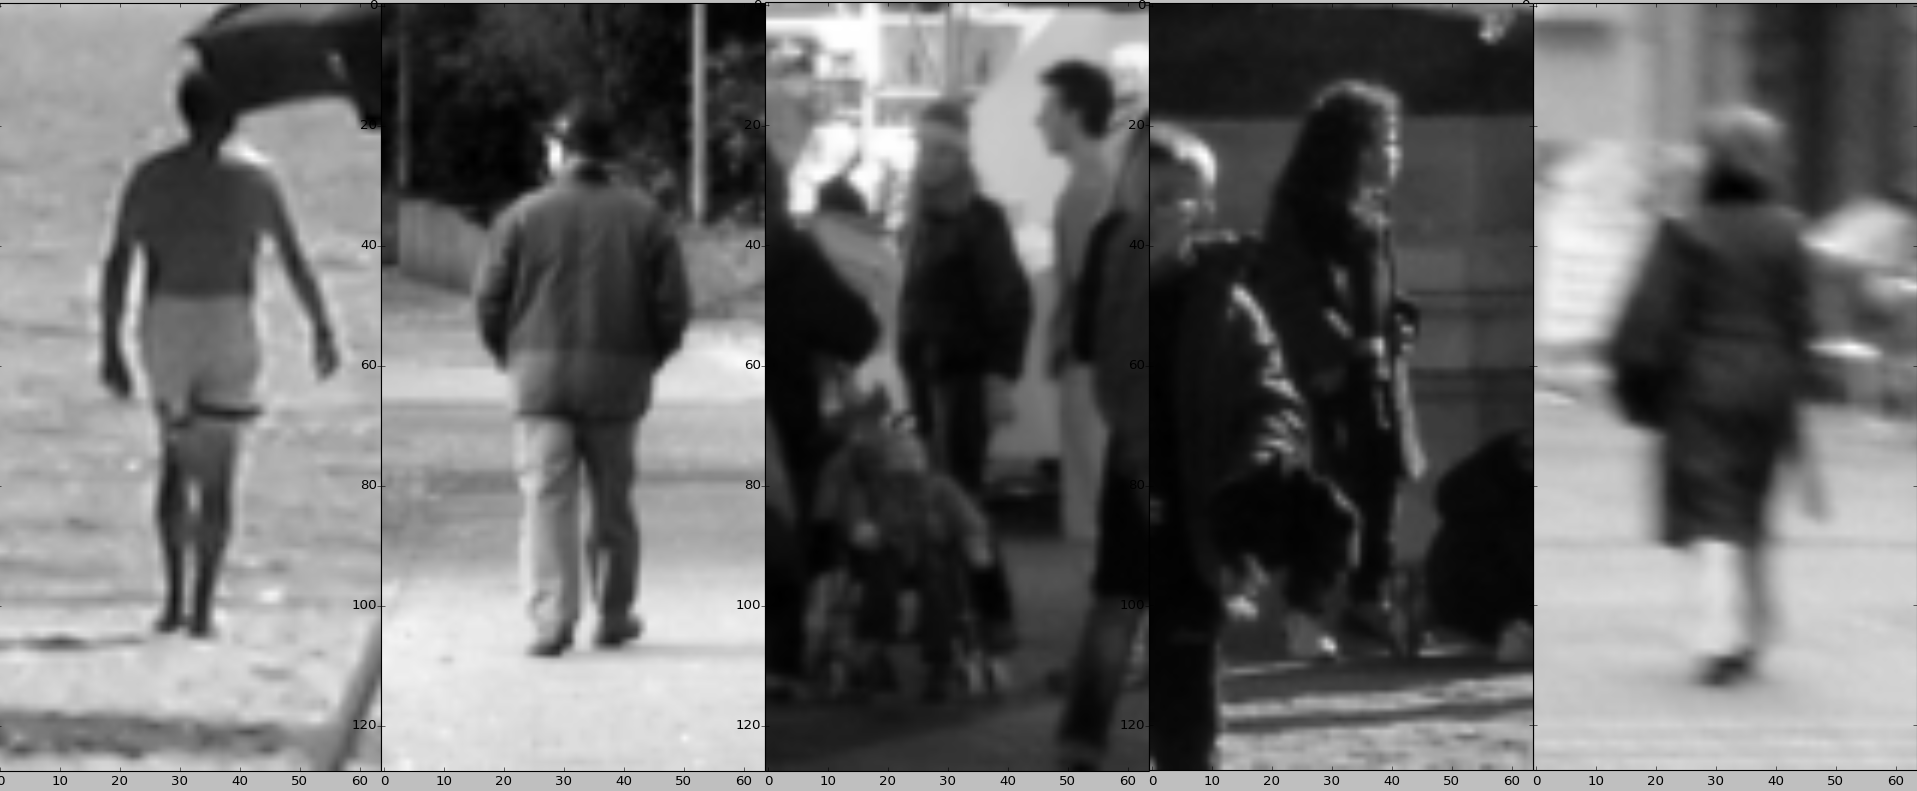
\includegraphics[width=0.93\textwidth]{imagini/exemplare_pozitive_inria_person.png}
	\caption{Exemplare pozitive din setul de date}
	\label{fig:exemplare_pozitive_inria_person}
\end{figure}


Antrenarea cu "bootstraping" a fost efectuata folosind 2500 de exemplare pozitive într-un număr de 10 iterații fiecare adăugând 1.000 de exemplare negative la modelul învățat. În total s-au folosit 10.000 de exemplare negative.

Lungimea vectorului de trăsături pentru o fereastra de dimensiune 64x128, folosindu-se celule de 8x8, blocuri de 16x16 și histograma cu 9 valori, este de 3870 de componente.

Factorul de scalare a piramidei de imagini este setat la 6/5 = 1.2, iar pasul ferestrei glisante este de 8 pixeli în ambele direcții.

În timpul antrenării modelul rezultat după fiecare iterație intermediara a fost salvat.

\subsection{Cod antrenament}
Codul programului de antrenare în Python este:
\lstinputlisting[language=Python]{cod_antrenament.py}

\subsection{Rezultate}
În continuare voi prezenta câteva rezultate ale algoritmului implementat.

\begin{figure}[H]
\begin{center}
	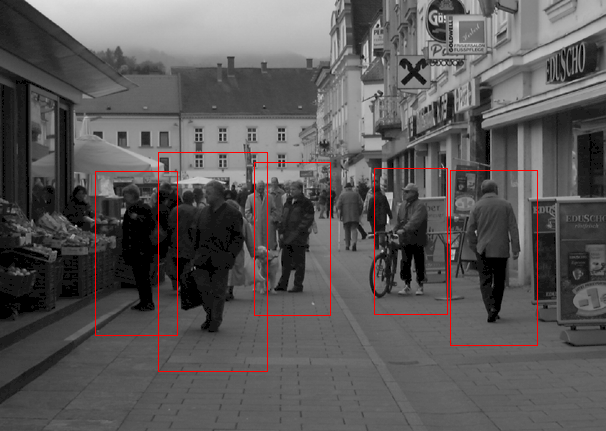
\includegraphics[width=1.00\textwidth]{imagini/rezultate_cu_nms.png}
\end{center}
	\caption{Rezultate recunoastere persoane}
	\label{fig:rezultate_recunoaster_pers1}
\end{figure}

\begin{figure}[H]
\begin{center}
	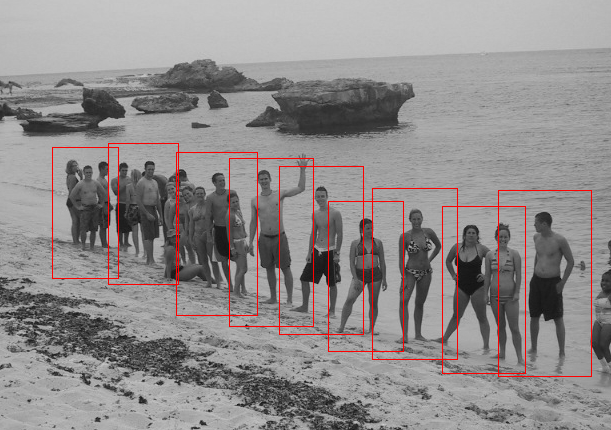
\includegraphics[width=1.00\textwidth]{imagini/rezultate2.png}
\end{center}
\begin{center}
	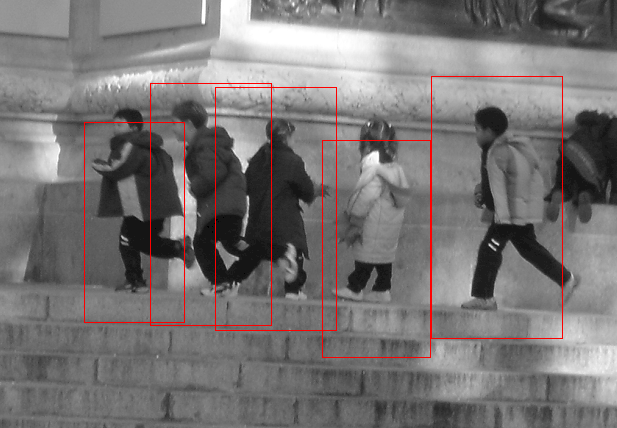
\includegraphics[width=1.00\textwidth]{imagini/rezultate3.png}
\end{center}
	\caption{Rezultate recunoastere persoane}
	\label{fig:rezultate_recunoaster_pers2}
\end{figure}

\subsection{Aplicație de recunoaștere a obiectelor}

În continuare voi prezenta aplicația de recunoaștere a obiectelor.

%Aplicația este una cu interfața grafica. Aceasta interfața a fost dezvoltata folosind biblioteca PySide.

Aceasta aplicație are rolul de a demonstra algoritmi de recunoaștere dezvoltați cu cadrul de lucru descris în aceasta lucrare.

Aplicația suporta următoarele operațiuni:
\begin{itemize}
	\item Încărcare și salvare algoritm
	\item Încărcare imagine
	\item Configurare parametrii algoritm
	\item Executarea algoritmului
\end{itemize}

Interfața cu utilizatorul a fost dezvoltata folosind biblioteca PySide și poate fi observata în figura \ref{fig:aplicatia}.

Un algoritm poate fi configurat cu ajutorul dialogului de configurare din figura \ref{fig:dialog_configurare}.

\begin{figure}[H]
	\centering
		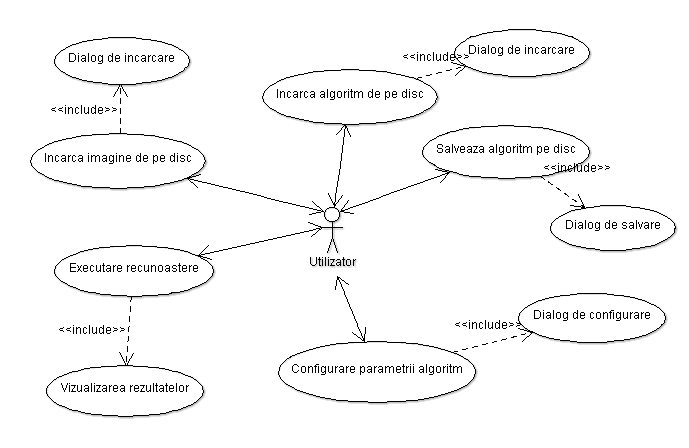
\includegraphics[width=1.00\textwidth]{uml/aplicatie_use_case.png}
	\caption{Diagrama Use Case a aplicatiei}
	\label{fig:aplicatie_use_case}
\end{figure}

\begin{figure}[H]
	\centering
		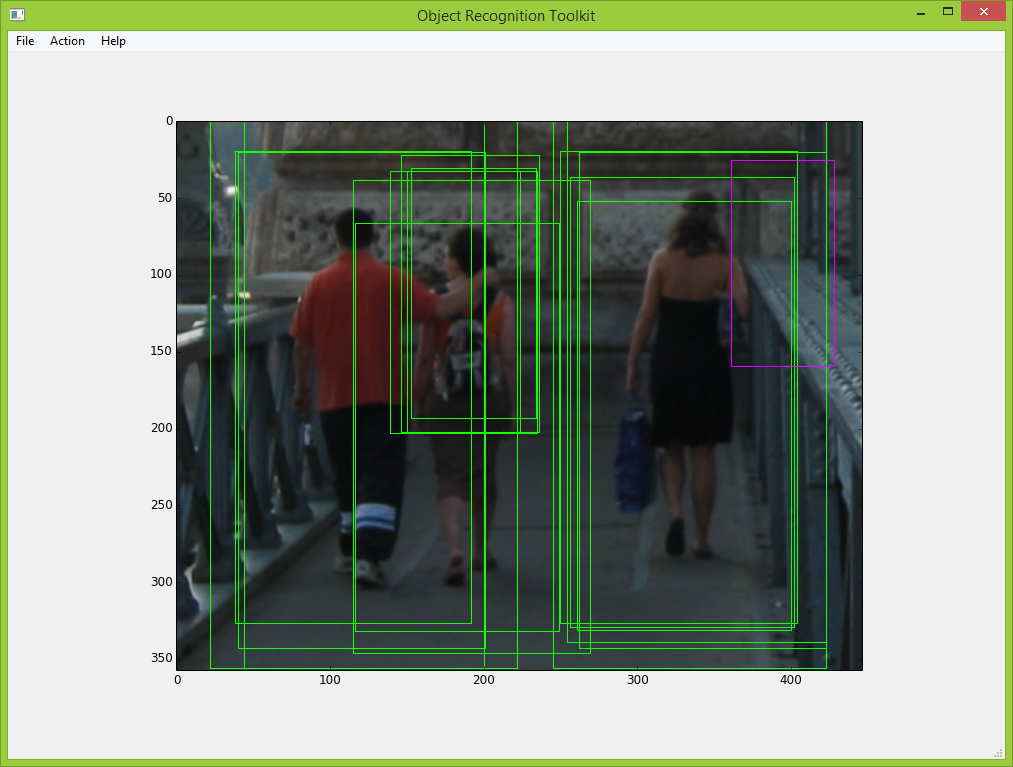
\includegraphics[width=1.00\textwidth]{imagini/aplicatia.png}
	\caption{Aplicatia de recunoastere}
	\label{fig:aplicatia}
\end{figure}

\begin{figure}[H]
	\centering
		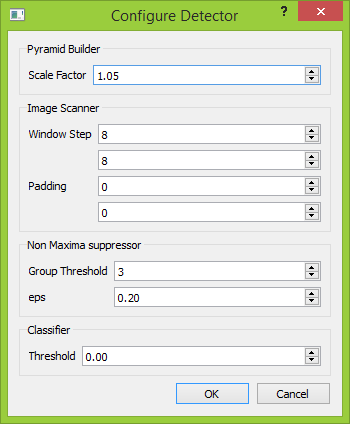
\includegraphics[width=0.45\textwidth]{imagini/dialog_configurare.png}
	\caption{Dialog de configurare}
	\label{fig:dialog_configurare}
\end{figure}


\section{Modalități de extindere a bibliotecii}

Scopul acestei lucrări este de a scurta timpul necesar dezvoltării algoritmilor de recunoaștere a obiectelor în imagini.
Acesta a fost realizat folosindu-se tehnici din programarea orientata pe obiecte.
Sunt proiectate interfețe și sunt oferite implementări pentru fiecare componenta a unui algoritm de recunoaștere.
Astfel, utilizatorul bibliotecii nu trebuie decât sa implementeze una sau doua componente pentru a obține un algoritm nou de recunoaștere.

Majoritatea algoritmilor de recunoaștere a obiectelor în imagini pot fi implementați folosind cadrul de lucru dezvoltat în aceasta lucrare. Diferențele apar doar la algoritmul de învățare automata sau de extragere a trăsăturilor.

\subsection{Exemplu}
O modalitate de extindere a unui algoritm este folosirea tehnicii de agregare.
Exemplu: adăugarea algoritmului PCA de reducere a dimensionalității la cel de învățare automata SVM.

\begin{figure}[H]
	\centering
		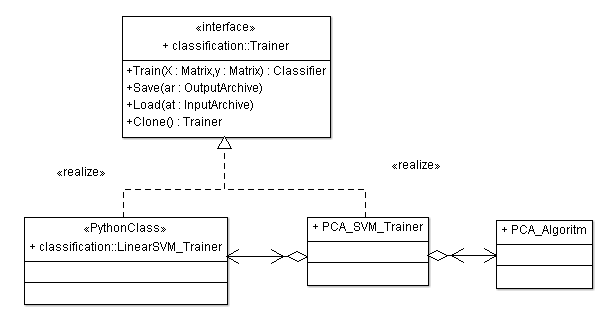
\includegraphics[width=0.90\textwidth]{uml/pca_classifier_diagram.png}
	\caption{Extindere algoritm de învățare automata}
	\label{fig:pca_classifier_diagram}
\end{figure}

Codul sursa pentru acest exemplu este:
\lstinputlisting[language=Python]{PCA_SVM_Trainer.py}

Urmărind acest exemplu se poate observa cat de ușor este de extins un algoritm folosind cadrul de lucru dezvoltat în aceasta lucrare.
Astfel de extinderi pot fi aplicate oricărei componente din algoritmul de recunoaștere.
%\section{Serializarea}

Serializarea are un rol important în dezvoltarea algoritmilor și aplicațiilor de recunoaștere a obiectelor.
Nu este nemaiîntâlnit ca antrenarea unui astfel de algoritm sa dureze zile întregi, de aceea este întotdeauna o idee buna ca rezultatul sau chiar pașii intermediari sa fie salvați pe disc, astfel evitând pierderea datelor.
Cele mai multe limbaje de programare moderne: Java, C\#, Python ne pun la dispoziție serializare obiectelor ca trăsătura de baza a limbajului.
C++, fiind un limbaj cu un sistem de tipuri foarte complex și fără management de memorie automat, nu deține facilitați de serializare automata.

Implementarea serializării în cadrul proiectului a fost realizata folosind biblioteca Boost.Serialization.
Am ales aceasta librărie datorita suportului pentru serializarea obiectelor polimorfice, o trăsătura necesara, data fiind natura orientata pe obiect în care a fost dezvoltat proiectul.

\pagebreak